\documentclass[usenames,dvipsnames,svgnames,table,aspectratio=169]{beamer}

\usepackage[utf8]{inputenc}
\usepackage{soul}
\usepackage{listings}
\usepackage{tikz}
\usepackage{booktabs}
\usepackage{minted}
\usepackage{biblatex}

\usetheme{laas}

\AtBeginSection[]{
  \begin{frame}
  \vfill
  \centering
  \begin{beamercolorbox}[sep=8pt,center,shadow=true,rounded=true]{title}
    \usebeamerfont{title}\insertsectionhead\par%
  \end{beamercolorbox}
  \vfill
  \end{frame}
}

\lstset{language=C++,
                basicstyle=\ttfamily,
                keywordstyle=\color{blue}\ttfamily,
                stringstyle=\color{red}\ttfamily,
                commentstyle=\color{purple}\ttfamily,
                morecomment=[l][\color{magenta}]{\#}
}


\title{Modern C++ Best Practices}
\author{Tim Luchterhand, based on a presentation by Paul Nykiel \cite{Nykiel2020}}
\date{\today}

\addbibresource{bibliography.bib}
\begin{document}
\maketitle

\frame{
    \tableofcontents
}

\section{Introduction}
\begin{frame}
    \frametitle{Features of C++}
    \begin{itemize}
        \item<+-> C++ $\neq$ C with classes!
        \item<+-> Deterministic lifetime of objects
        \item<+-> No garbage collection
        \item<+-> Undefined behavior
    \end{itemize}
\end{frame}

\begin{frame}
    \frametitle{Object Lifetime}
    \lstinputlisting{examples/slides/lifetime.cpp}
\end{frame}

\begin{frame}
    \frametitle{Memory Leak}
    \lstinputlisting{examples/slides/memory_leak.cpp}
\end{frame}

\begin{frame}
    \frametitle{General Goals}
    \begin{itemize}
        \item<+-> Avoid undefined behavior at all times
        \item<+-> Let go of old habits from C, do not use C constructs if not necessary
        \begin{itemize}
            \item<+-> C-Arrays
            \item<+-> Pointers
            \item<+-> Manual memory management
        \end{itemize}
        \item<+-> Focus on logic instead of low level data structures and memory management
        \item<+-> Use the STL
    \end{itemize}
\end{frame}

\section{Memory Layout}
\begin{frame}
    \frametitle{Stack and Heap}
    \begin{columns}
        \begin{column}{.5\textwidth}
            \begin{itemize}
                \item<+-> System memory (RAM) is divided in two parts
                \item<+-> Stack is used for function calls
                \item<+-> Heap is used for dynamically allocated memory
                \item<+-> Allocated memory on the heap needs to be freed \textit{manually}
                \item<+-> If there is more than one owner this can get complicated
            \end{itemize}
        \end{column}
        \begin{column}{.5\textwidth}
            \begin{figure}[H]
                \centering
                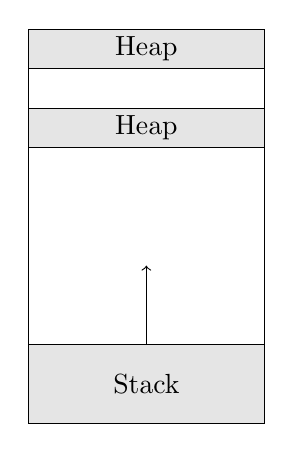
\begin{tikzpicture}
                    \draw [draw] (0,0) rectangle (3,5);
                    \filldraw [draw=black,fill=gray!20] (0,0) rectangle (3,1) node[pos=.5] {Stack};
                    \filldraw [draw=black,fill=gray!20] (0,4.5) rectangle (3,5) node[pos=.5] {Heap};
                    \filldraw [draw=black,fill=gray!20] (0,3.5) rectangle (3,4) node[pos=.5] {Heap};
                    \draw [->] (1.5,1) -- (1.5,2);
                \end{tikzpicture}
            \end{figure}
        \end{column}
    \end{columns}
\end{frame}

\begin{frame}
    \frametitle{Example: Stack}
    \begin{columns}
        \begin{column}{.5\textwidth}
            \lstinputlisting{examples/slides/stack.c}
        \end{column}
        \begin{column}{.5\textwidth}
            \begin{figure}[H]
                \centering
                \only<1> {
                    \begin{tikzpicture}
                        \draw [draw] (0,0) rectangle (3,6);
                    \end{tikzpicture}
                }
                \only<2,6> {
                    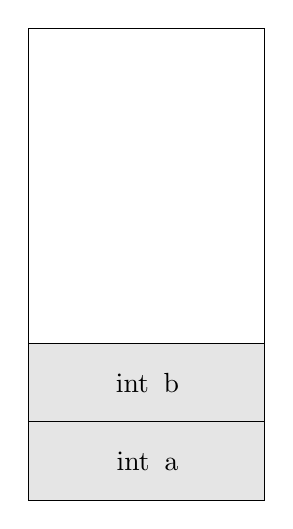
\begin{tikzpicture}
                        \draw [draw] (0,0) rectangle (3,6);
                        \filldraw [draw=black,fill=gray!20] (0,0) rectangle (3,1) node[pos=.5] {\lstinline{int a}};
                        \filldraw [draw=black,fill=gray!20] (0,1) rectangle (3,2) node[pos=.5] {\lstinline{int b}};
                    \end{tikzpicture}
                }
                \only<3> {
                    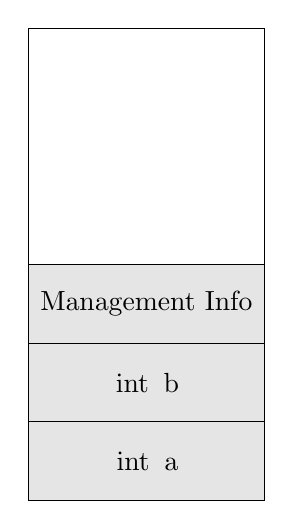
\begin{tikzpicture}
                        \draw [draw] (0,0) rectangle (3,6);
                        \filldraw [draw=black,fill=gray!20] (0,0) rectangle (3,1) node[pos=.5] {\lstinline{int a}};
                        \filldraw [draw=black,fill=gray!20] (0,1) rectangle (3,2) node[pos=.5] {\lstinline{int b}};
                        \filldraw [draw=black,fill=gray!20] (0,2) rectangle (3,3) node[pos=.5] {Management Info};
                    \end{tikzpicture}
                }
                \only<4> {
                    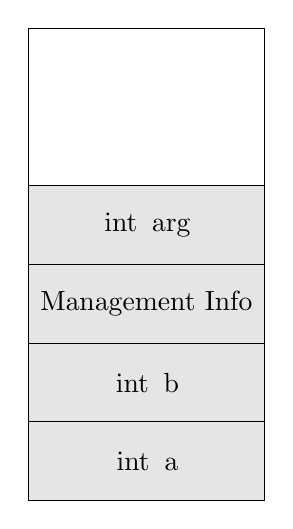
\begin{tikzpicture}
                        \draw [draw] (0,0) rectangle (3,6);
                        \filldraw [draw=black,fill=gray!20] (0,0) rectangle (3,1) node[pos=.5] {\lstinline{int a}};
                        \filldraw [draw=black,fill=gray!20] (0,1) rectangle (3,2) node[pos=.5] {\lstinline{int b}};
                        \filldraw [draw=black,fill=gray!20] (0,2) rectangle (3,3) node[pos=.5] {Management Info};
                        \filldraw [draw=black,fill=gray!20] (0,3) rectangle (3,4) node[pos=.5] {\lstinline{int arg}};
                    \end{tikzpicture}
                }
                \only<5> {
                    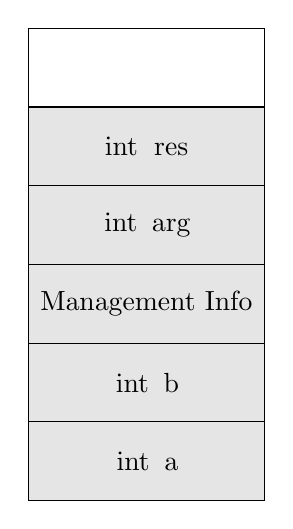
\begin{tikzpicture}
                        \draw [draw] (0,0) rectangle (3,6);
                        \filldraw [draw=black,fill=gray!20] (0,0) rectangle (3,1) node[pos=.5] {\lstinline{int a}};
                        \filldraw [draw=black,fill=gray!20] (0,1) rectangle (3,2) node[pos=.5] {\lstinline{int b}};
                        \filldraw [draw=black,fill=gray!20] (0,2) rectangle (3,3) node[pos=.5] {Management Info};
                        \filldraw [draw=black,fill=gray!20] (0,3) rectangle (3,4) node[pos=.5] {\lstinline{int arg}};
                        \filldraw [draw=black,fill=gray!20] (0,4) rectangle (3,5) node[pos=.5] {\lstinline{int res}};
                    \end{tikzpicture}
                }
            \end{figure}
        \end{column}
    \end{columns}
\end{frame}

\begin{frame}
    \Huge{Is that not enough?}
\end{frame}

\begin{frame}
    \frametitle{Example: Heap}
    \begin{columns}
        \begin{column}{.5\textwidth}
            \lstinputlisting{examples/slides/heap.cpp}
        \end{column}
        \begin{column}{.5\textwidth}
            \begin{figure}[H]
                \centering
                \only<1> {
                    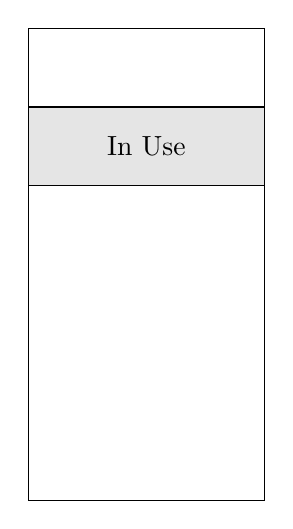
\begin{tikzpicture}
                        \draw [draw] (0,0) rectangle (3,6);
                        \filldraw [draw=black,fill=gray!20] (0,5) rectangle (3,4) node[pos=.5] {In Use};
                    \end{tikzpicture}
                }
                \only<2> {
                    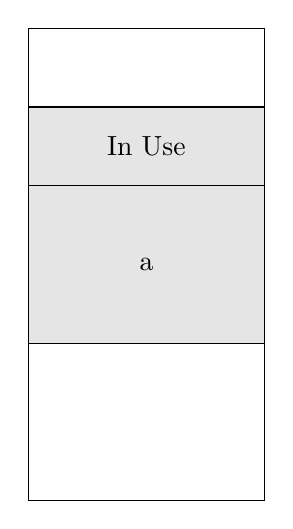
\begin{tikzpicture}
                        \draw [draw] (0,0) rectangle (3,6);
                        \filldraw [draw=black,fill=gray!20] (0,5) rectangle (3,4) node[pos=.5] {In Use};
                        \filldraw [draw=black,fill=gray!20] (0,4) rectangle (3,2) node[pos=.5] {\lstinline{a}};
                    \end{tikzpicture}
                }
                \only<3> {
                    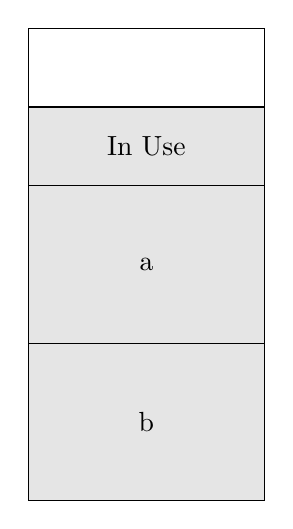
\begin{tikzpicture}
                        \draw [draw] (0,0) rectangle (3,6);
                        \filldraw [draw=black,fill=gray!20] (0,5) rectangle (3,4) node[pos=.5] {In Use};
                        \filldraw [draw=black,fill=gray!20] (0,4) rectangle (3,2) node[pos=.5] {\lstinline{a}};
                        \filldraw [draw=black,fill=gray!20] (0,2) rectangle (3,0) node[pos=.5] {\lstinline{b}};
                    \end{tikzpicture}
                }
                \only<4> {
                    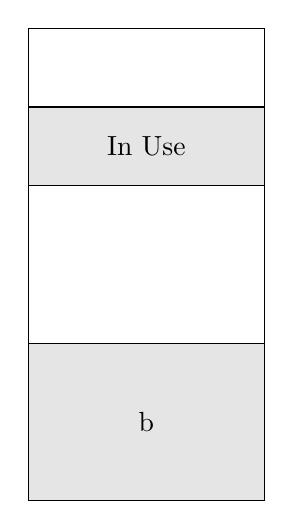
\begin{tikzpicture}
                        \draw [draw] (0,0) rectangle (3,6);
                        \filldraw [draw=black,fill=gray!20] (0,5) rectangle (3,4) node[pos=.5] {In Use};
                        \filldraw [draw=black,fill=gray!20] (0,2) rectangle (3,0) node[pos=.5] {\lstinline{b}};
                    \end{tikzpicture}
                }
            \end{figure}
        \end{column}
    \end{columns}
\end{frame}


\section{Zero Copy: Function Parameters and Smart-Pointers}
\begin{frame}
    \frametitle{C++ Copies by Default}
    \begin{itemize}
        \item<+-> \lstinputlisting{examples/slides/copy.cpp}
        \item<+-> \textit{Every} assignment is a copy
        \item<+-> Very simple
        \item<+-> Bad Performance for large objects
    \end{itemize}
\end{frame}

\begin{frame}
    \frametitle{Pass by Reference}
    \lstinputlisting{examples/slides/references.cpp}
\end{frame}

\begin{frame}
    \frametitle{Smart-Pointers}
    \begin{itemize}
        \item<+-> Substitute for "raw C-pointers"
        \item<+-> Standard library takes care of memory management
        \item<+-> \lstinline{std::unique\_ptr}
        \begin{itemize}
            \item<+-> exactly one owner (cannot be copied) 
            \item<+-> frees memory at destruction
            \item<+-> \lstinline{std::unique\_ptr<int> ptr = std::make\_unique<int>(17);}
        \end{itemize}
        \item<+-> \lstinline{std::shared\_ptr}
        \begin{itemize}
            \item<+-> multiple owners
            \item<+-> a bit like reference types in Java or C\#
            \item<+-> fees memory once all owning pointers have been destroyed
            \item<+-> \lstinline{std::shared\_ptr<int> ptr = std::make\_shared<int>(17);}
        \end{itemize}
        \item<+-> \lstinline{std::weak\_ptr} to avoid shared pointer cycles
    \end{itemize}
\end{frame}

\begin{frame}
    \frametitle{Shared Pointer Example}
    \lstinputlisting{examples/slides/shared_ptr.cpp}
\end{frame}

\section{Move Semantics}
\begin{frame}
    \frametitle{Introduction}
    \begin{itemize}
        \item<+-> Introduced with C++ 11
        \item<+-> Allows to transfer resources from one owner to another
        \item<+-> \lstinline|std::move|
        \item<+-> all std containers support moving
    \end{itemize}
\end{frame}

\begin{frame}
    \frametitle{Simple Example}
    \lstinputlisting{examples/slides/move.cpp}
\end{frame}

\begin{frame}
    \frametitle{Another Example}
    \lstinputlisting{examples/slides/move1.cpp}
\end{frame}

\begin{frame}
    \frametitle{When is a Move Performed Automatically?}
    \lstinputlisting{examples/slides/when_moved.cpp}
\end{frame}

\begin{frame}
    \frametitle{What Happens if we Move an Object}
    \lstinputlisting{examples/slides/move_explanation.cpp}
\end{frame}

\begin{frame}
    \frametitle{What does std::move do?}
    Quote from cppreference.com:
    
    It is exactly equivalent to a \lstinline|static\_cast| to an rvalue reference type. 
    \pause
    \lstinputlisting{examples/slides/move_impl.cpp}
\end{frame}

\section{Rule of Zero, Rule of Five, RAII}

\begin{frame}
    \frametitle{Special Members}
    \begin{itemize}
        \item<+-> Copy constructor \lstinline{Object(const Object o &other)}
        \item<+-> Move constructor \lstinline{Object(Object o &&other)}
        \item<+-> Copy assignment \lstinline{Object &operator=(const Object &other)}
        \item<+-> Move assignment \lstinline{Object &operator=(Object &&other)}
        \item<+-> Destructor \url{~}\lstinline{Object()}
    \end{itemize}
\end{frame}

\begin{frame}
    \frametitle{Rule of Zero}
    \begin{itemize}
        \item<+-> Classes that do not directly manage memory
        \item<+-> Compiler auto-generates all five special members (memberwise)
        \item<+-> Rule (cpp core guidelines): \textbf{If you can avoid defining default operations, do!}
    \end{itemize}
    \only<+->{\lstinputlisting{examples/slides/rule_of_zero.cpp}}
\end{frame}

\begin{frame}
    \frametitle{Rule of Five}
    \begin{itemize}
        \item<+-> Classes that manage resources need to
        \begin{itemize}
            \item<+-> free them in the Destructor
            \item<+-> make sure that copy construction and assignment are carried out correctly
        \end{itemize}
        \item<+-> Move constructor and assignment are disabled if any of the following members is given
        \begin{itemize}
            \item<+-> Copy constructor (even \lstinline|= default| or \lstinline|= delete|)
            \item<+-> Copy assignment (even \lstinline|= default| or \lstinline|= delete|)
            \item<+-> Destructor (even \lstinline|= default|)
        \end{itemize}
        \item<+-> Rule: \textbf{If you define any of the five special members, define them all!}
    \end{itemize}
\end{frame}

\begin{frame}
    \frametitle{Rule of Five}
    \lstinputlisting{examples/slides/rule_of_five.cpp}
\end{frame}


\begin{frame}
    \frametitle{Resource Acquisition is Initialization (RAII)}
    \begin{itemize}
        \item<+-> Classes that manage resources acquire them during initialization (constructor)
        \item<+-> Destructor cleans everything up
        \item<+-> Provides exception safety
    \end{itemize}
    \only<+->{\lstinputlisting{examples/slides/raii.cpp}}
\end{frame}

\begin{frame}
    \frametitle{Extension}
    After a call to the constructor, \textbf{any} object should be ready to use. Bad example:
    \pause
    \lstinputlisting{examples/slides/raii1.cpp}
\end{frame}

\section{Useful Tools and Refernces}
\begin{frame}
    \frametitle{Address Sanitizer}
    \begin{itemize}
        \item<+-> Detects invalid memory accesses and memory leaks
        \item<+-> Works with clang and g++
        \item<+-> Add compilation flag \lstinline{-fsanitize=address -g}
    \end{itemize}
\end{frame}

\begin{frame}
    \frametitle{backwardscpp}
    \begin{itemize}
        \item<+-> Header only library \url{https://github.com/bombela/backward-cpp}
        \item<+-> Prints readable stack traces
        \item<+-> Best integrated with CMake
    \end{itemize}
\end{frame}

\begin{frame}
    \frametitle{Clang-Tidy}
    \begin{itemize}
        \item<+-> Static code analysis tool \url{https://clang.llvm.org/extra/clang-tidy/}
        \item<+-> Detects bugprone and inefficient code
        \item<+-> Checks can be configured in config file
        \item<+-> Directly integrated in CLion
    \end{itemize}
\end{frame}

\begin{frame}
    \frametitle{Useful References}
    \begin{itemize}
        \item<+-> \url{cppreference.com}
        \begin{itemize}
            \item<+-> Official documentation of the stl
            \item<+-> Core language features and properties
            \item<+-> Examples
        \end{itemize}
        \item<+-> Cpp Core guidelines: \url{https://isocpp.github.io/CppCoreGuidelines/CppCoreGuidelines}
        \begin{itemize}
            \item<+-> C++ philosophy
            \item<+-> \textbf{Best practices}
        \end{itemize}
        \item<+-> \url{godbolt.org} compiler explorer
        \begin{itemize}
            \item<+-> Collection of all compilers
            \item<+-> Assembly view
        \end{itemize}
    \end{itemize}
\end{frame}

\begin{frame}
    \frametitle{What is Missing?}
    \begin{itemize}
        \item<+-> Best practices:
        \begin{itemize}
            \item<+-> Const correctness
            \item<+-> Error handling
            \item<+-> Operator overloading
            \item<+-> Function design: in, in-out and out parameters
            \item<+-> Code documentation
        \end{itemize}
        \item<+-> Language / library features
        \begin{itemize}
            \item<+-> Templates and meta programming
            \item<+-> Lambdas
            \item<+-> Ranges
            \item<+-> Concurrency and multi-threading
        \end{itemize}
    \end{itemize}

    

\end{frame}

\section*{References}
\begin{frame}
  \frametitle{This Work is Strongly Inspired and Based on}
  \printbibliography
\end{frame}

\end{document}
